
Conceptual overview of software architecture and its parts is given on figure \ref{fig:soft_overview}. All components will be discussed and described in detail in this section of the report. 

%\begin{figure}[th!]
%\center
%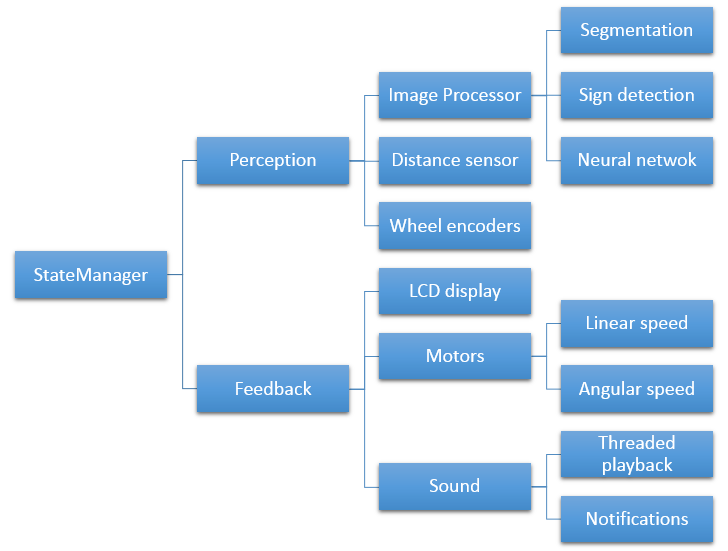
\includegraphics[scale=0.7]{images/software-architecture.png}
%\caption{Overview of software architecture of the solution}
%\end{figure}


\begin{figure}[!ht]
	\hspace{-1cm}
	\begin{tikzpicture}[node distance = 2.5cm, auto]
	% % % % % % % % % % % % % % % % % % % % % % % % % % % % % %
	% Define styles
	\tikzstyle{block} = [rectangle, draw, fill=blue!20, text width=5em, text centered, 
					     rounded corners, minimum height=3em, font=\small]
	\tikzstyle{line} = [draw, -latex', line width =2pt]
	
	% % % % % % % % % % % % % % % % % % % % % % % % % % % % % %
	% Place nodes
	% parent
	\node [block,  fill=blue!40] (sm) {State Manager};
	% child level 1
	\node [block, fill=blue!35, below of=sm, node distance = 1.7 cm, xshift=-4.cm] (pc) {Perception};
	\node [block, fill=blue!35, below of=sm, node distance = 1.7 cm, xshift=4.cm] (fb) {Feedback};
	% child level 2 left
	\node [block, below of=pc, node distance = 1.7cm] (ds) {Distance sensor};
	\node [block, left of=ds] (ip) {Image Processor};
	\node [block, right of=ds,  node distance = 2.5 cm] (we) {Wheel encoders};
	% %third level left
	\node [block, below of=ip, node distance = 1.7 cm] (sgd) {Sign detection};
	\node [block, left of=sgd] (sgm) {Sign Segmentation};
	\node [block, right of=sgd] (nn) {Neural network};
	
	% child level 2 right
	\node [block, below of=fb, node distance = 1.7 cm] 						(ld) {LCD display};
	\node [block, left of=ld] 	(sn) {Sound};
	\node [block, right of=ld] (mt) {Motors};
	
	% %third level right
	\node [block, below of=sn, node distance = 1.7 cm, xshift=-1.25cm] (ntf) {Notifications};
	\node [block, below of=sn, node distance = 1.7 cm, xshift=1.25cm] (thr) {Threaded playback};
	% %third level right
	\node [block, below of=mt, node distance = 1.7 cm, xshift=-1.25cm] (lns) {Linear speed};
	\node [block, below of=mt, node distance = 1.7 cm, xshift=1.25cm] (ags) {Angular speed};
	
%	\node [block, right of=left,  node distance = 3 cm] (right) {Turn right};
	% Draw edges
	\path [line] (sm) -- (fb);
	\path [line] (sm) -- (pc);
	% %
	\path [line] (pc) -- (ip);
	\path [line] (pc) -- (we);
	\path [line] (pc) -- (ds);
	% %
	\path [line] (fb) -- (sn);
	\path [line] (fb) -- (mt);
	\path [line] (fb) -- (ld);
	% %  third level image proc
	\path [line] (ip) -- (sgm);
	\path [line] (ip) -- (sgd);
	\path [line] (ip) -- (nn);
	% %  third level sound
	\path [line] (sn) -- (ntf);
	\path [line] (sn) -- (thr);
	% %  third level motors
	\path [line] (mt) -- (lns);
	\path [line] (mt) -- (ags);
	\end{tikzpicture}
	\caption{Overview of software architecture of the solution}
	\label{fig:soft_overview}
\end{figure}

